\chapter{Methods} \label{methods}
This Chapter contains a thoroughly description of the methods followed during this thesis work. Firstly, a characterization of the case is provided. It contains the description of the settings, the case itself and the units of analysis. Subsequently, the focus shifts to the methods and sources through which the data has been collected. For every different source the text describes where applicable use cases and rationale. Finally, the chapter ends with an explanation of the data analysis methods used. 


%
%
% START CASE DESCRIPTION
%
%
\section{Case Definition}	\label{sec:case-description}
To answer the research questions defined in Chapter \ref{sec:introduction} this study will use the \textit{Holistic Exploratory Case Study} research methodology as described by \cite{case_study_guide}. Furthermore, the guidelines expressed by Runeson and H{\"o}st \cite{case_study_software_engineering} has been taken into consideration; they specifically target the Software Engineering field with a detailed checklist which is possible to find in appendix \ref{checklist_for_case_studies} with links to the relevant parts of this report.


For properly characterize the Case under study Yin \cite{case_study_guide} suggests to describe 1) the context in which the Case is, 2) the Case itself, and 3) the Units of Analysis used during the study.

As for number 1, this study took place in the Swedish office of the Company, which globally employs more than 3000 people scattered in several offices. Its core business is licensing software products for managing personnel and equipments in the context of Transportation. The portfolio offers different solutions to cover several business needs in terms of short or long term planning, personnel optimization etc.

Internally, teams use Scrum for managing their development activities. They have great freedom in choosing sprint length, and the Definition of Done, which is build on top of a minimum one provided by the parent company. Teams are cross functional and hence contain people with different areas of expertise; they also are self-contained meaning that they should carry out all software related activities independently.

This last fact is of great relevance for this study. In fact, all testing activities are carried on separately, following the minimum guidelines expressed in the Definition of Done. However, this lenient artifact causes teams to use different testing strategies for complying with testing pipeline. Therefore, there is a chance to witness the accruing of TD from different perspectives. 

As shown in Fig. \ref{fig:testing_pipeline}, this pipeline is composed of four main levels (lower to higher): unit tests, components tests, system tests, end to end tests. These levels do not differentiate between functional and quality (non-functional) testing types as these can take place at any level. 

Particularly, unit tests are carried on by developers alongside development activities and aim to test the System at function / class level. Therefore, there is a high number of them and tend to be fast to execute and fairly simple. At this level, developers follow the same guidelines specified for the actual source code, with the sole exception that, according to the minimum definition of done, they are not reviewed. Above in the hierarchy there are component tests which target interaction between macro software-entities and aim to ensure that the sub-parts of the system deliver the desired functionality. At this level the target are the exposed APIs and not the internal mechanics of the source code. The next level in the pipeline is composed by system tests which aim to assure that user functionality and business processes of a single system comply with the specification. These tests are executed at user interface level with realistic data sets and possibly data volume. Furthermore, the system is cloned from production environments. Finally, End to End tests are similar in concept and execution to System tests, but they test the interaction of two or more complete systems.

\todo{Improve figure \ref{fig:testing_pipeline} readability}
\todo{Extract the image from the testing chapter document}

\begin{figure}[ht]
    \centering
    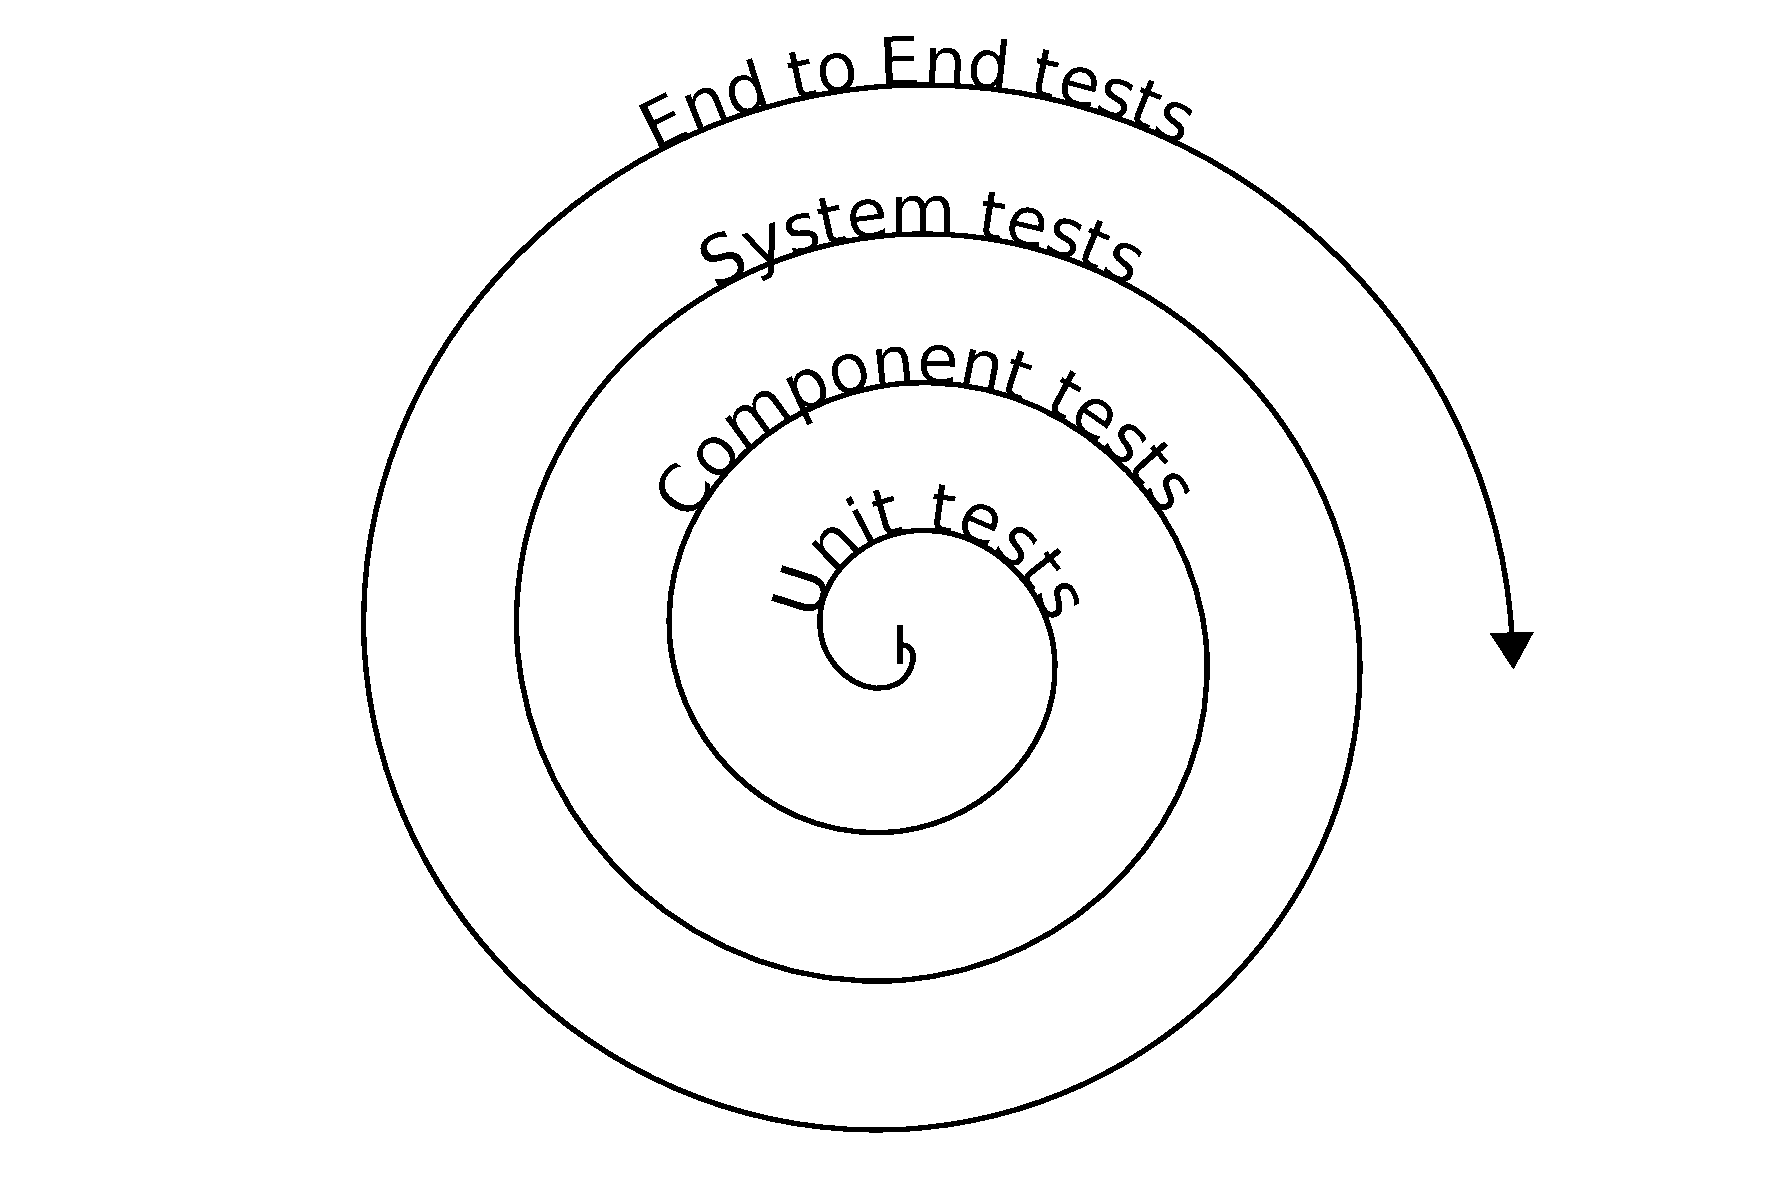
\includegraphics[width=\textwidth]{figure/testing_pipeline.pdf}
    \caption{Testing pipeline in use at the Company}
    \label{fig:testing_pipeline}
\end{figure}

To properly framing the inquiry the chosen \textit{Cases} are the projects that use Hewlett Packard UFT (Unified Functional Test) for GUI testing (formerly known as QTP) both for smoke testing and for regression testing. This tool allows testers to mix Property Based GUI testing with Image Recognition GUI testing. Within these projects I will evaluate the maintenance activities that target the two higher testing levels of the functional part of the mentioned pipeline. Specifically how much extra maintenance derives from the use of bad code practices used in GUI test scripts. With that said, the chosen \textit{Unit of Analysis} are the such maintenance activities. 
    

%
%
% END CASE DESCRITPION
%
%

%
%
% START DATA GATHERING
%
%
\section{Data Gathering}
As recommended by \cite{case_study_guide,case_study_software_engineering}, data has been gathered from various sources in order to increase Data Triangulation and hence improve the reliability of the study. These sources are: 1) informal interviews (a.k.a.\ coffee machine / water bowl interviews), 2) the company´s forum, 3) the company´s issue tracker and backlog, 4) the repositories of the relevant project, and 5) semi-structured interviews.

However, some of the data sources just assisted the inquiry conducted by other methods; i.e.\ informal interviews and forum were used during the first phase the study to delimit the inquiry conducted through other sources like the analysis of the repositories.

Finally, considering the extensive amount of data that has been generated, it has proven impossible to insert the raw results in any part of the report. Instead, it is available on-line at \href{http://???/}. However, readers should be aware that the raw data was anonymized and every sensitive information was also removed. 

\todo{Insert link to thesis database}
\todo{Mention that data is 3rd stage}
\todo{Mention that I used both quantitative and qualitative sources for improving reliability}

\subsection{Informal Interviews}
This source helped defining the scope of the inquiry in the first stages of the study by identifying at very high level main problems and triggering causes. However, due to the lack of repeatability associated with this method, such data has not been used for sensitive parts of the study like theory validation.

In fact, the frequency, the location, and the interviewee were random. They occurred during lunch and/or coffee breaks whenever possible. Furthermore, the topics covered were not willful and depended on current issues encountered by the interviewee. Anyhow, their importance during the first phases of this study is clear since focused the attention on important parts, sources, and documentation.

\subsection{Mining of The Forum} \label{mining_forum}
In order to enable Knowledge Sharing the company adopted Confluence, a collaborative software / forum developed and maintained by Atlassian, which allows technical and non-technical employers to share procedures, ideas, and comments in an asynchronous fashion. For this reason this source is valuable since it contains numerous information, which can shed light on the problems this Thesis aim to study.

However, considering the magnitude of the available data, the mining has been done through a systematic approach using the embedded search engine followed by two manual filtering steps to ensure that no relevant information were missed. In fact, the system contains data covering several years and include several thousands discussions threads and many more answers. 

The keywords entered in the search engine were included in double quotes in order to enable the \textit{exact match} feature. This choice was needed to limit the number of results to a manageable size. For instance, \textit{test maintenance} yielded 8467 results whereas \textit{"test maintenance"} 28. Subsequently, the first coarser temporal based filter followed. It eliminated hits older than one year. Next, the second finer filter was used. It is based on the relevance. Finally, the remaining set of posts has been carefully read and pertinent ones has been anonymized and transcribed in the Thesis database. Table \ref{tab:confluenceMiningResults} the results obtained for each step for the keywords used.

This paragraph reports the rationale connected with the first filtering activity. The temporal time frame is narrow for two reasons. Firstly, the testware stack has changed during last year (2014) and hence the findings could be biased by information not relevant or dependant to the old technologies. Secondly, the mortality of the resources has been taken into account. In fact, the Company greatly relies on consultants and their turnover is shorter than normal employees. 

\subsection{Mining of The Issue Tracker / Backlogs}
The Company uses an all in one solution for managing issues and their Agile Environments: JIRA + JIRA Agile Plugin which are also managed by Atlassian. Similarly to the forum this source contains a high number of entries that have been filtered before being analyzed and included in this study evidence. However, the filtering process has been tailored to consider the different nature of these entries.

In fact, the descriptive text inserted in \textit{user stories} or \textit{issues} is more concise than the one found in the forum. Moreover, the entries simply consist of a list of actions. Some entries, however, contain a rationale which tend to be slightly more verbose, but still succinct. 

For this reason the decision of only using \textit{``UFT''} as keyword has been taken and  the resulting entry set has been filtered only based on relevance since the number of result yielded by the query was manageable.

However, due to the highly sensitive information about issues, bugs, and planned features included in this source I cannot disclose any part of them and hence I limit to report the the keywords used with the raw numbers.


\subsection{Analysis of The Repositories} \label{analysis_of_the_repos}
The company extensively uses \textit{Concurrent Versions System}. At the time of writing their system contains 870 repositories of various size belonging to 20 different projects in a many-to-many relationship. The company also deployed two different tools to browse such repositories with ease: \textit{HgWeb} and \textit{Crucible + FishEye}. They are migrating to the second one since it also allows asynchronous code reviews and can be integrated with the Issue Tracker and the Forum since part of the suite developed by Atlassian.

Given the amount of data contained in this archival source, the data coming from other sources was used to select the subset of repositories that better suites the goal of this Thesis; I.e.\ a selected number of repositories targeting test code that are currently under active development or maintenance.

\todo{Finishing this section describing what I did with the commits when I will actually perform the mining}

\subsection{Semi-Structured Interviews} \label{semi-structured_interviews}
During this study total of \inote{Number of Interviews here} semi-structured interviews was conducted; they follow the guidelines expressed in \cite{interview_guideline}. The decision to use this interview format derives from the need to have a good degree of flexibility to adapt the inquiry while maintaining the scope constrained.

The purpose of this data source was two-fold: to provide  some insights during the first phase of the study, and to validate the findings during the final one. In fact, the first interview was used to gain awareness about the testing situation within the Company whereas the others were the remaining ones validate the theory proposal crafted after analyzing the other data sources. Furthermore, they also created open questions for future studies on the topic.

\todo{Finish the subsection describing settings, who has been interviewed and such
}



%
%
% END DATA GATHERING
%
%


%
%
% START DATA INTERPRETATION
%
%
\section{Interpretation of the Data} \label{data_interpretation}

The interpretation of the data plays a key role in experimental studies like this one. Furthermore, analyzing both qualitative sources (e.g.\ Forum) and quantitative ones (e.g.\ Repositories) requires an approach that successfully melds together these different sources. For this reason, I believe that using \textit{Coding} \cite{qualitative_inquiry} for qualitative inquiry and \textit{Pattern matching} \cite{case_study_guide} for a quantitative data is the best approach.

The approach followed in this study relies on both methods concurrently. In fact, I used the coding practices in the first part of the study, aiming to extrapolate recurrent patterns and problems from different sources which in turn allowed me to narrow the scope. Subsequently, through pattern matching I create a first theory draft that has been revised with more qualitative inquiry. Finally, through semi-structured interviews, I validated such theory with the help of practitioners.

The two following subsections thoroughly describe the mentioned approaches, however the results are reported in Chapter \ref{study_results}.

\subsection{Coding}
In this study I followed the three coding techniques described by Corbin and Strauss \cite{coding_guidelines}. Namely 1) open coding, 2) axial coding, and 3) selective coding. Furthermore, these tasks were aided by \href{http://www.qsrinternational.com/products_nvivo.aspx}{NVivo 10 for Windows} which allow to manage the coding process with ease.

Open coding is used to analytically break down data and its purpose is to gain new insight about the phenomenon by using non-conventional interpretation criteria. During this process the data fragments are conceptually labeled and similar ones tied together. This creates categories and sub-categories that can be broken down in even finer items such as properties and characteristics. This intensive fracturing of the data forces the researcher to examine preexisting ideas against a very detailed representation of data itself and hence it eliminates subjectivity and bias.

In axial coding the researcher test the connection between categories and sub-categories against the data by analyzing connections, consequences, and conditions. Furthermore, during this step there is a further development of the categories created during open coding. It is recommended to alternate the collection and analysis of the data throughout the study since the analysis phase can guide with more precision the data gathering activities.

Selective coding is the stage in which categories are connected to a \textit{core category} that represents the phenomenon under study. This core category can be identified by asking questions like: \textit{``what does all the action/interaction seem to be about?''}, \textit{``How can I explain all the variation I see among categories?''}, etc.\ \cite{coding_guidelines}. It is obvious that this stage must takes place in the later phases of the study.

Finally, I am going to describe how these coding phases have been carried out during the study. The first open coding iteration took place after six weeks since prior to that the data was too scarce. Afterwards every time one of the data sources described before was exploited, I went through the open coding and axial coding as recommended and hence  I continuously improved the categories previously created. Finally, I performed the Selective coding in \tocite{Enter week number when the selective coding has been performed}.


\subsection{Pattern matching}
Yin \cite{case_study_guide} and Trochim \cite{pattern_matching} consider Pattern matching as one of the best approaches to meld together existing theories with the data gathered within a study. Furthermore, it eases the evaluation of rival theories since a it allows to rule them out thanks to the fitness with the discovered pattern \cite{pattern_matching}.

In this Thesis, the pattern was extrapolated from the Repositories and matched against quantitative and qualitative models provided by the literature. For obvious reasons, in the latter case the inference conducted has been solely inductive, meaning that the findings associated are not corroborated by statistical weight and hence might lack external validity.

\todo{Select wich pattern matching I will use (need to read the paper more carefully)}

Trochim \cite{pattern_matching} highlights several pitfalls that must be considered when using this technique; otherwise the power of this method is greatly hindered. 

Firstly, the conceptualization of the model must be appropriate, e.g.\ using formulae to describe a purely qualitative model is a bad practice since constants derive from the researcher best guesses.

Secondly, the level of generalization of the formulated pattern must match the purpose of the study and the study and the desired level of generalization.

Third, pattern formulation tend to be more effective when performed without prior knowledge of the observed pattern. In fact, the researcher judgment could be biased by this prior knowledge. Fact that inflated the threats to reliability and internal validity.

Next, the holistic perspective that researchers tend to use while performing pattern matching could exclude relevant details. This specially applies when pattern are extracted from a set of metrics or measures.

Finally, when measuring the fitness of patterns using statistical methods their analytical accuracy with respect to the context in which are embedded must be considered in order to avoid false positive results.


\todo{Expand these risks and measures taken to avoid them in validity threats section}